% This is LLNCS.DEM the demonstration file of
% the LaTeX macro package from Springer-Verlag
% for Lecture Notes in Computer Science,
% version 2.4 for LaTeX2e as of 16. April 2010
%
\documentclass{llncs}
%
\usepackage{makeidx}  % allows for indexgeneration
\usepackage[utf8]{inputenc}
\usepackage{graphicx}
%
\begin{document}
%
\frontmatter          % for the preliminaries
%
\pagestyle{headings}  % switches on printing of running heads
\addtocmark{Eternity II} % additional mark in the TOC
%

\mainmatter              % start of the contributions
%
\title{Solving Eternity II Redux\\
	\small{An approach based on Genetic Algorithms}
}
%
\titlerunning{Eternity II - Genetic Algorithms Approach}  % abbreviated title (for running head)
%                                     also used for the TOC unless
%                                     \toctitle is used
%
\author{João Gradim \and Mário Carneiro}
%
\authorrunning{João Gradim\inst{1} et Mário Carneiro\inst{1}} % abbreviated author list (for running head)
%
%%%% list of authors for the TOC (use if author list has to be modified)
\tocauthor{João Gradim and Mário Carneiro}
%
\institute{Faculdade de Engenharia da Universidade do Porto,\\
\email{ei05030@fe.up.pt}, \email{ei04051@fe.up.pt}}

\maketitle              % typeset the title of the contribution

\begin{abstract}
%TODO: o abstract escreve-se no fim.
Eternity II is an NP-complete edge-matching puzzle which solution has not yet been discovered. This article, we will describe how it is possible to tackle this problem by using genetic algorithms.
\end{abstract}
%
\section{Introduction}\label{sec:introduction}

%This section will describe why we are picking up on the work previously developed by Fábio Aguiar and Sara Carvalho, and what methodologies we will try

The Eternity II puzzle is an edge-matching puzzle. It consists of a 16 by 16 grid that must be completed with the respective 256 pieces. Each piece has four coloured patterns on its edges. The tiles are placed on a 16x16 board and can be freely rotated before being placed.

%TODO: inserir aqui imagens bonitas do puzzle

A solution is found when all of the edges match their neighboring tiles' edges. The puzzle was conceived specifically so it is very difficult to solve by brute force searching methods. The puzzle was designed as a competition by Christopher Monckton in 2005. A two million US dollars prize is being offered to the first complete solution of this puzzle.

% TODO: cite http://www.prnewswire.co.uk/cgi/news/release?id=188486

Our work was toward solving smaller versions of this puzzle - with less edge patterns and a board of smaller dimensions.


%Our work will be in the direction of improving known methods ideal for solving smaller versions - with less pieces, less patterns and a board of smaller dimensions - of this puzzle. The reason for this is that no method has yet been found that can solve the original puzzle, at least in a feasible time span.

%We will pick up on the work developed by Fábio Aguiar and Sara Carvalho in this same context. This article will document exactly where we began, what possible improvements could be applied to the previous work, as well the results we hope to achieve and the results we've got.

We will also use an existing element to base our work upon: The \textit{Eternity II Editor} is an open-source Java-based application that allows the creation and edition of Eternity II puzzle grids. \textit{Eternity II Editor}'s features include a series of puzzle solving programs and the ability to see the program's attempt to solve the puzzle in real time. More importantly, it features a usable application interface that will allow us to extend the application with out own solving methods.

\section{Problem Description}\label{sec:problem_description}

\subsection{Eternity II puzzle description}\label{sec:puzzle_description}

The Eternity II puzzle is an edge-matching puzzle. Solving the puzzle means placing the puzzle's 256 square pieces on a 16 by 16  grid in such a way that all of the pieces' edges match adjacent edges. The puzzle was designed to be difficult to solve by brute-force computer search, as there are roughly $1.115 * 10 ^ {557}$ possible configurations.

\begin{figure}[h]
	\centering
	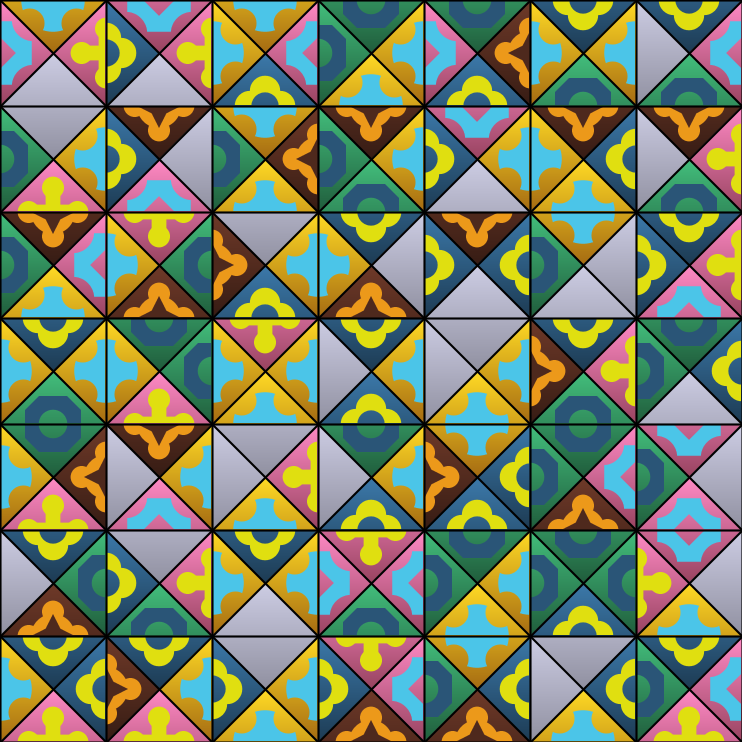
\includegraphics[width=35mm]{images/shuffled.png}
	\caption{Simplified puzzle with 7 by 7 tiles, with 6 colors}
	\label{fig:shuffled_example}
\end{figure}

\begin{figure}[h]
	\centering
	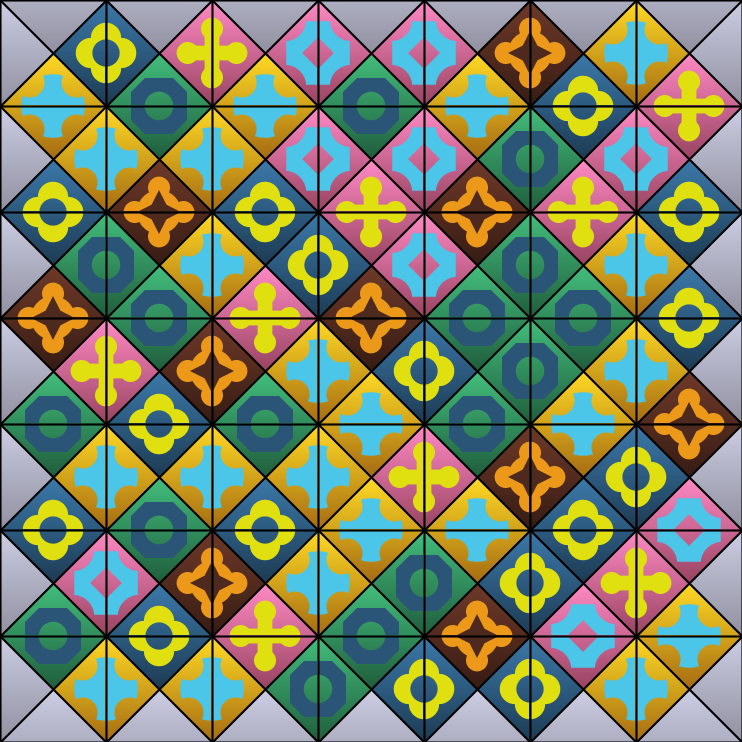
\includegraphics[width=35mm]{images/solved.png}
	\caption{Solution to the above puzzle}
	\label{fig:solved_example}
\end{figure}

Each piece has its edges marked with different shape and colour combinations, henceforth called patterns. Each must precisely match the neighboring piece's edge when the puzzle is solved. These pieces can also be placed in four different positions, by rotating them 90º, 180º or 270º. Pieces that will sit on a corner or borderline tile can be easily distinguished from all the other, as they have a grey edge. There are 22 different patterns in the original puzzle (excluding the grey edges).

\subsection{Normal approaches to solving the problem}\label{sec:normal_approaches}

We have found that the most common approaches that solve these kinds of problems can fall into one of two types: swap and iterative. Swap solutions always start with a complete board, and then use the rotate and swap operations in order to improve the board's state. Iterative approaches place pieces progressively, according to a certain criteria and can backtrack to any previous state if they determine that no good solution will be found from that point onward.

\subsubsection{The swap approach}\label{sec:swap_approach}

As said before, swap approaches begin by placing all the available pieces in the board, then use the swap and rotate operations to improve the board's state. There are plenty algorithms that can achieve this, like hill-climbing, tabu search and simulated annealing. These approaches evaluate the board's state and try to find which sequence of operations will achieve the greatest score possible (which in turn will lead to a solved puzzle).

Evidently, the starting position of the pieces in the puzzle will also play an important part on the rest of the solving process. (Explain why?)

\subsubsection{The iterative approach}\label{sec:iterative_approach}

Iterative solutions try to place the pieces progressively, usually following some kind of pattern.
(Describe here most common patterns that can be used.)

\section{Approaching Eternity II with Genetic Algorithms}\label{sec:genetic_algorithms}

\subsection{Introducing: The Genetic Algorithm}
(Methodologies and approaches taken when trying new methods to improve solving times of The desired simplified Eternity II puzzles)

A genetic algorithm (\textit{GA}, for short) is an uninformed search method that mimics the process of natural evolution. It is particularly useful in search and optimization problems. The genetic algorithm works by generating solutions using procedures inspired by natural evolution: Search begins on a set, called \textit{population} of initial states, called \textit{individuals or chromosomes}. The characteristics that make up each individual can therefore be thought of \textit{genetic material}. The quality of the solution each individual represents is measured by a problem-specific \textit{fitness} function. Evolution of the population (and consequently of the best solution) is achieved by \textit{selection} and \textit{reproduction} betwen individuals of the population, often in some respect to their fitness evaluation. This creates new individuals in the population whose genetic material comes from individuals in the previous generation.
\textit{Mutations} in the individuals are often introduced betwen generations so that we can diverge from the set that contains all possible combinations of genetic material present in the initial population, which may or may not include the solution sought after.

These kind of algorithms have been proven useful in solving many kinds of problems, including puzzle problems. A textbook example of an application of GA's is the \textit{n-queens} problem\cite{eastridge}.

\subsection{Methodology}\label{sec:methodology}

% FIXME: tá péssimo
\subsubsection{Individuals and Population}
Solving Eternity II with \textit{GA}'s implies that we must first choose the state that will represent our known solutions in the search space. Our state, or in the context of \textit{GA}'s', \textit{individual} or \textit{chromosome} is the trivial solution to this problem: the board itself.
The initial state in our search problem is the unsolved board. It defines exactly the size and characteristics of the problem: The problem size and the set of pieces that will be present in all individuals of the population.
Our initial population of $n$ individuals is built from random shuffling of the initial state $n$ times.

\subsubsection{Fitness function}\label{sec:fitness-function}

The fitness function used to evaluate the quality of the boards is given by:

\begin{figure}[h]
	\begin{equation}
		fitness = \frac{n\_matching\_edges}{total\_matching\_edges}
	\end{equation}
	\caption{Fitness function for evaluating boards}
	\label{fig:eq:fitness_function}
\end{figure}

where \textit{n\_matching\_edges} represents the number of matching edges between all pieces of the board for the current state, and \textit{total\_matching\_edges} the number of matching edges for an $n*n$ board. As such, \textit{fitness} will yield a value between $[0.0, 1.0]$, with higher values corresponding to fitter boards. A fitness of exactly $1.0$ would only be attributed to a board that is correctly solved.

\subsubsection{Breeding}\label{sec:breeding}

Starting out with \textit{n} random permutations of the same board, the fittest half of the population is selected for breeding, using an ?elitist? selection approach. These specimens are then bred and their genetic code is crossed-over according to very specific rules:

\begin{itemize}
	\item If both parents have compatible features, use both features on both descendants in order to create fitter boards
	\item If both parents have incompatible features, select the highest scoring feature from each parent and use it as a starting point for each of the descendants
	\item The rest of the genetic code (pieces) not originated from the feature selection is then placed on the descendant boards using a simple (no backtracking) linear constructive method
	\item Mutations are then performed on a random set of pieces by rotating them in order to try and improve the overall fitness of the board
\end{itemize}

\subsubsection{Mutations}\label{sec:mutations}

After each reproduction each new individual suffers a series of mutations (with a probability of 50\%). These mutations are piece-oriented, and are performed by selecting $n-1$ random pieces (where $n$ corresponds to the size of the board) and rotating them clockwise. This approach provides solid results, until the board score nears its maximum: when this situation arises, the solution becomes stagnant due to the fact that only one or two pieces need to be rotated to achieve a correct solution. To overcome this problem, when the board score reaches a certain threshold ($score >= maximum score - 4$), all board pieces are checked and rotated (if necessary), in order to maximize the number of connections, providing a correct solution in most observed cases.

\subsection{Implementation}\label{sec:implementation}

\subsubsection{Feature Extraction}\label{sec:feature_extraction}

\subsubsection{Eternity II Editor}\label{sec:eternity2_editor}

(Why are we using Eternity II Editor and how we linked the previously developed solution with it)

\section{Results}\label{sec:results}

(Experimental results obtained from the application of the new methodologies to the diamonds board approach)

\section{Conclusions}\label{sec:conclusions}

(Conclusions go here)
%
% ---- Bibliography ----
%
\bibliographystyle{plain}
\bibliography{mpes}
\end{document}

